
\section{Grundlagen}
\subsection{Überwachtes Lernen}
\newcommand\yhat{\,\hat{y}}
\newcommand\Yhat{\, \hat{Y}}

The common ground for all further aspects in this work will be supervised learning, which is most generally speaking simply the task of deriving a function from data. This function should be able to map given inputs or data points to some sort of output. In the supervised setting, data is given with an associative label such, that the inferred function is able to map said input data to the correct labels, without explicitly looking at the given labels. The learning algorithm, when deriving said function, therefore has to use patterns and structure among the data points to learn something about the quality of a given data point. Outputs are generally either of a quantitative type e.g. temperature measurements or changes in stock price or of a qualitative type like distinctive types of flowers. Tasks involving the former kinds of outputs are generally referred to as regression problems whereas the tasks involving the latter are generally called classification problems.
\\We can roughly articulate the supervised learning problem as follows: for a given input $X$, an associated label $Y$ and a function $ \mathbb{F}(X)= \Yhat$, $\mathbb{F}$ makes a good prediction, when $\Yhat$ is close to $Y$. Proximity, in this case, must be defined and can vary depending on the type of data which is present. For a regression problem of e.g. predicting tomorrows temperature, the prediction is better, the more similar the predicted value $\Yhat$ and tomorrows true temperature are, measured by the absolute distance of $|Y-\Yhat|$.
X in this case could be a vector of meteorologic measurements which are regarded highly predictive of short term weather prognosis.
\subsubsection{Lineare Modelle}
Linear Regression has been a staple in statistics and machine learning and remains a very important and widely used tool \cite{hastie01statisticallearning}. As it serves as the basis for a wide range of more complex machine learning algorithms like logistic regression and in some sense even Deep Neural Networks, it serves as a good introduction. The linear model 
\begin{align*}
\mathbb{F}(X) =  \beta + \sum_{i=1}^{|X|}w_ix_i = \yhat
\end{align*} 
predicts Y by using a linear combination of all input variables $x_i$ using weights $w_i$. $\beta$ is the intercept of the linear decision boundary, often referred to as the bias. Since in this case we are modeling a scalar value, $\yhat$ is a single value, but can also be N-vector if we're predicting values of higher dimensionality. To get an idea how good our model is performing, we first need to come up with a way of measuring its prediction quality. The sum of squares is a widely used method and sums each squared difference between any predicted value $\yhat_i$ and its corresponding true value $y_i$. We define the sum of squared errors as $E$, a function of our parameters $\mathbb{W}$ which we then can minimize. Since it is a quadratic function, its minimum always exists but does not have to be unique.
\begin{align*}
E(\mathbb{W}) = \frac{1}{2}\sum_{i=1}^{N}(\yhat_i - y_i)^2 =
\frac{1}{2}\sum_{i=1}^{N}(\sum_{j=1}^{|X|}(w_ix_i + \beta) - y_i)^2
\end{align*}
Minimizing E($\mathbb{W})$ with respect to $\mathbb{W}$ yields:
\begin{align*}
\frac{\delta E}{\delta \mathbb{W}} =  \left(\frac{\delta E}{\delta w_1 },...,\frac{\delta E}{\delta w_n }\right) = \left( \sum_{i=1}^{N}(\yhat_i - y_i)x_1,...,\sum_{i=1}^{N}(\yhat_i - y_i)x_n \right)
\end{align*}
\subsection{Biologischer Hintergrund}
Das menschliche Gehirn kann Probleme wie Bild- und Spracherkennung in erstaunlicher Zeit und ohne für den Menschen ersichtliche Mühe Lösen. Probleme, die für Computer, trotz ihrer weitaus überlegenen Rechenkraft, in der Vergangenheit schwer bis unlösbar waren. Was das menschliche Gehirn neben seinen über 100 Milliarden Neuronen ausmacht, ist die Strukturelle Ordnung in hochkomplex organisierte Netzwerke. Um diese Neuronalen Netzwerke zu verstehen, müssen einige Grundlagen über einzelne Neuronen gelegt werde.
\subsection{Neuronen}
\label{sec:neurons}
\begin{wrapfigure}{R}{0.4\textwidth}
	\centering
	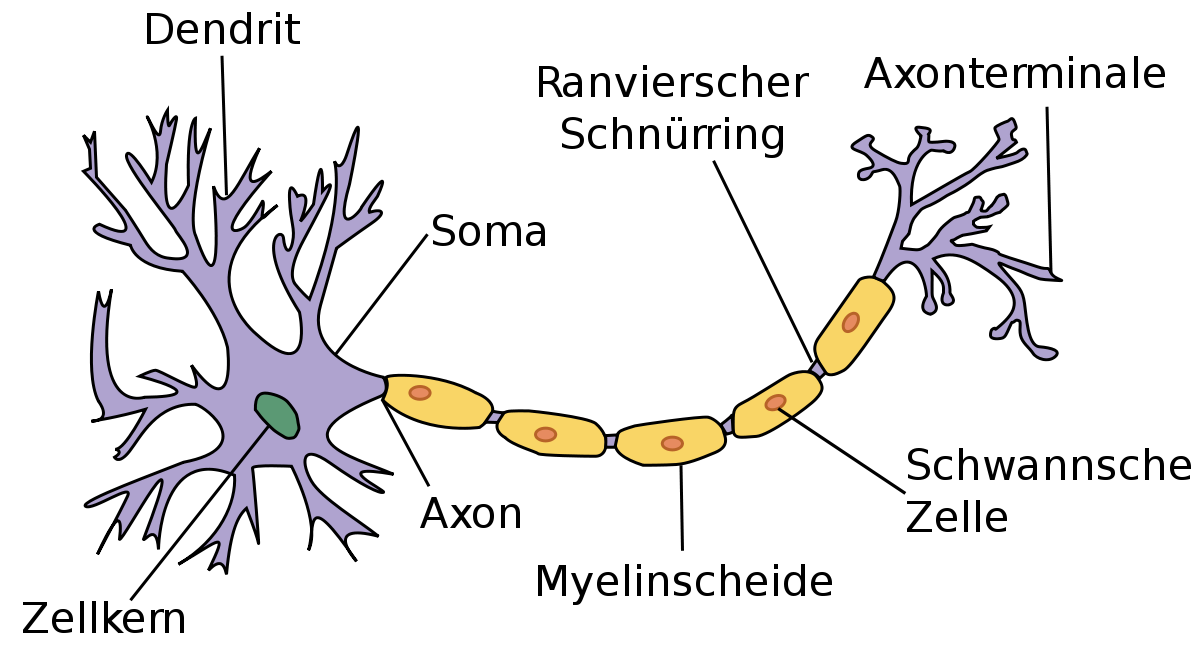
\includegraphics[width=0.35\textwidth]{abb/neuron.png}
	\caption{Schematische Darstellung eines Neurons}
\end{wrapfigure}
Neuronen (auch: Nervenzellen) sind die Grundeinheit des Nervensystems. Sie sind auf Signalweiterleitung spezialisierte Zellen und ähneln anderen Zellarten, weil sie ebenso einen Zellkern, eine Zellmembran und andere Organellen wie Mitochondrien besitzen. Die verschiedenen Arten solcher Neuronen haben grundsätzlich eine dreiteilig Architektur gemeinsam: sie bestehen aus den Dendriten, dem Soma und einem Axon. Dendriten sind Zellfortsätze aus dem Soma der Nervenzelle, die diffus verzweigen und nur bis wenige Mikrometer entfernt vom Soma reichen. Sie dienen hauptsächlich der Reizaufnahme und leiten eingehende Reize zum Zellkörper weiter. Das Soma ist 4 bis 100 Mikrometer groß, der Körper oder das Zentrum der Zelle und enthält Zellkern und andere Organellen, die für eine normale Zellfunktion nötig sind. Am Axonhügel des Somas verankert beginnt das Axon, ein dünner, fadenartiger Fortsatz, der das Signal der Nervenzelle weiterleitet und in seinen Endregionen, den Synapsen, mit anderen Zellen, wie Nerven-, Muskel- oder Drüsenzellen in Verbindung steht. Eine einzelne Nervenzelle dabei kann bis zu 10000 Synapsen besitzen.\par
\begin{wrapfigure}{L}{0.4\textwidth}
	\centering
	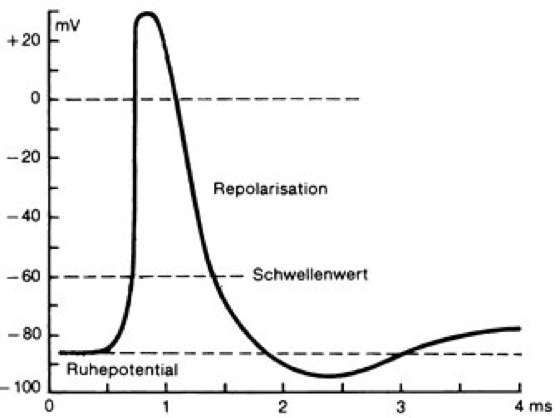
\includegraphics[width=0.35\textwidth]{abb/ap.jpg}
	\caption{Spannungsänderung während eines Aktionspotentials}
\end{wrapfigure}
Die wichtigste Grundlage der Kommunikation von Neuronen sind Aktionspotentiale, welche entstehen, wenn das Membranpotential eines Axons sehr schnell fluktuiert. Im Ruhezustand weisen Nervenzellen ein Membranpotential von -70mV bis -80mV auf, wobei eine solche elektrische Spannung zwischen dem intra- und dem extrazellulären Raum durch das Aufrechterhalten einer Ungleichverteilung von elektrisch geladenen Teilchen (Ionen) entsteht. Die Ionenkanäle, die für dieses Ungleichgewicht verantwortlich sind, reagieren selbst auf elektrische Spannung und verändern ihre Durchlässigkeit in Abhängigkeit der Spannung. Ändert sich das Membranpotential am Axonhügel durch eingehende Signale, welche beispielsweise von anderen Neuronen über die Dendriten ins Soma propagiert werden, über einen gewissen Grenzwert, entsteht eine Veränderung in der Permeabilität der Ionenkanäle, die eine Kettenreaktion am Axon hervorrufen. Dabei entstehen lokale Depolarisierungen, die das Membranpotential um 100mV anheben und in benachbarten Regionen denselbe Effekt hervorrufen. Das so entstehende elektrische Signal wandert am Axon entlang in die Synapsen, wo es beispielsweise an die Dendriten anderer Nervenzellen weitergeleitet wird. \par
\begin{wrapfigure}{R}{0.4\textwidth}
	\centering
	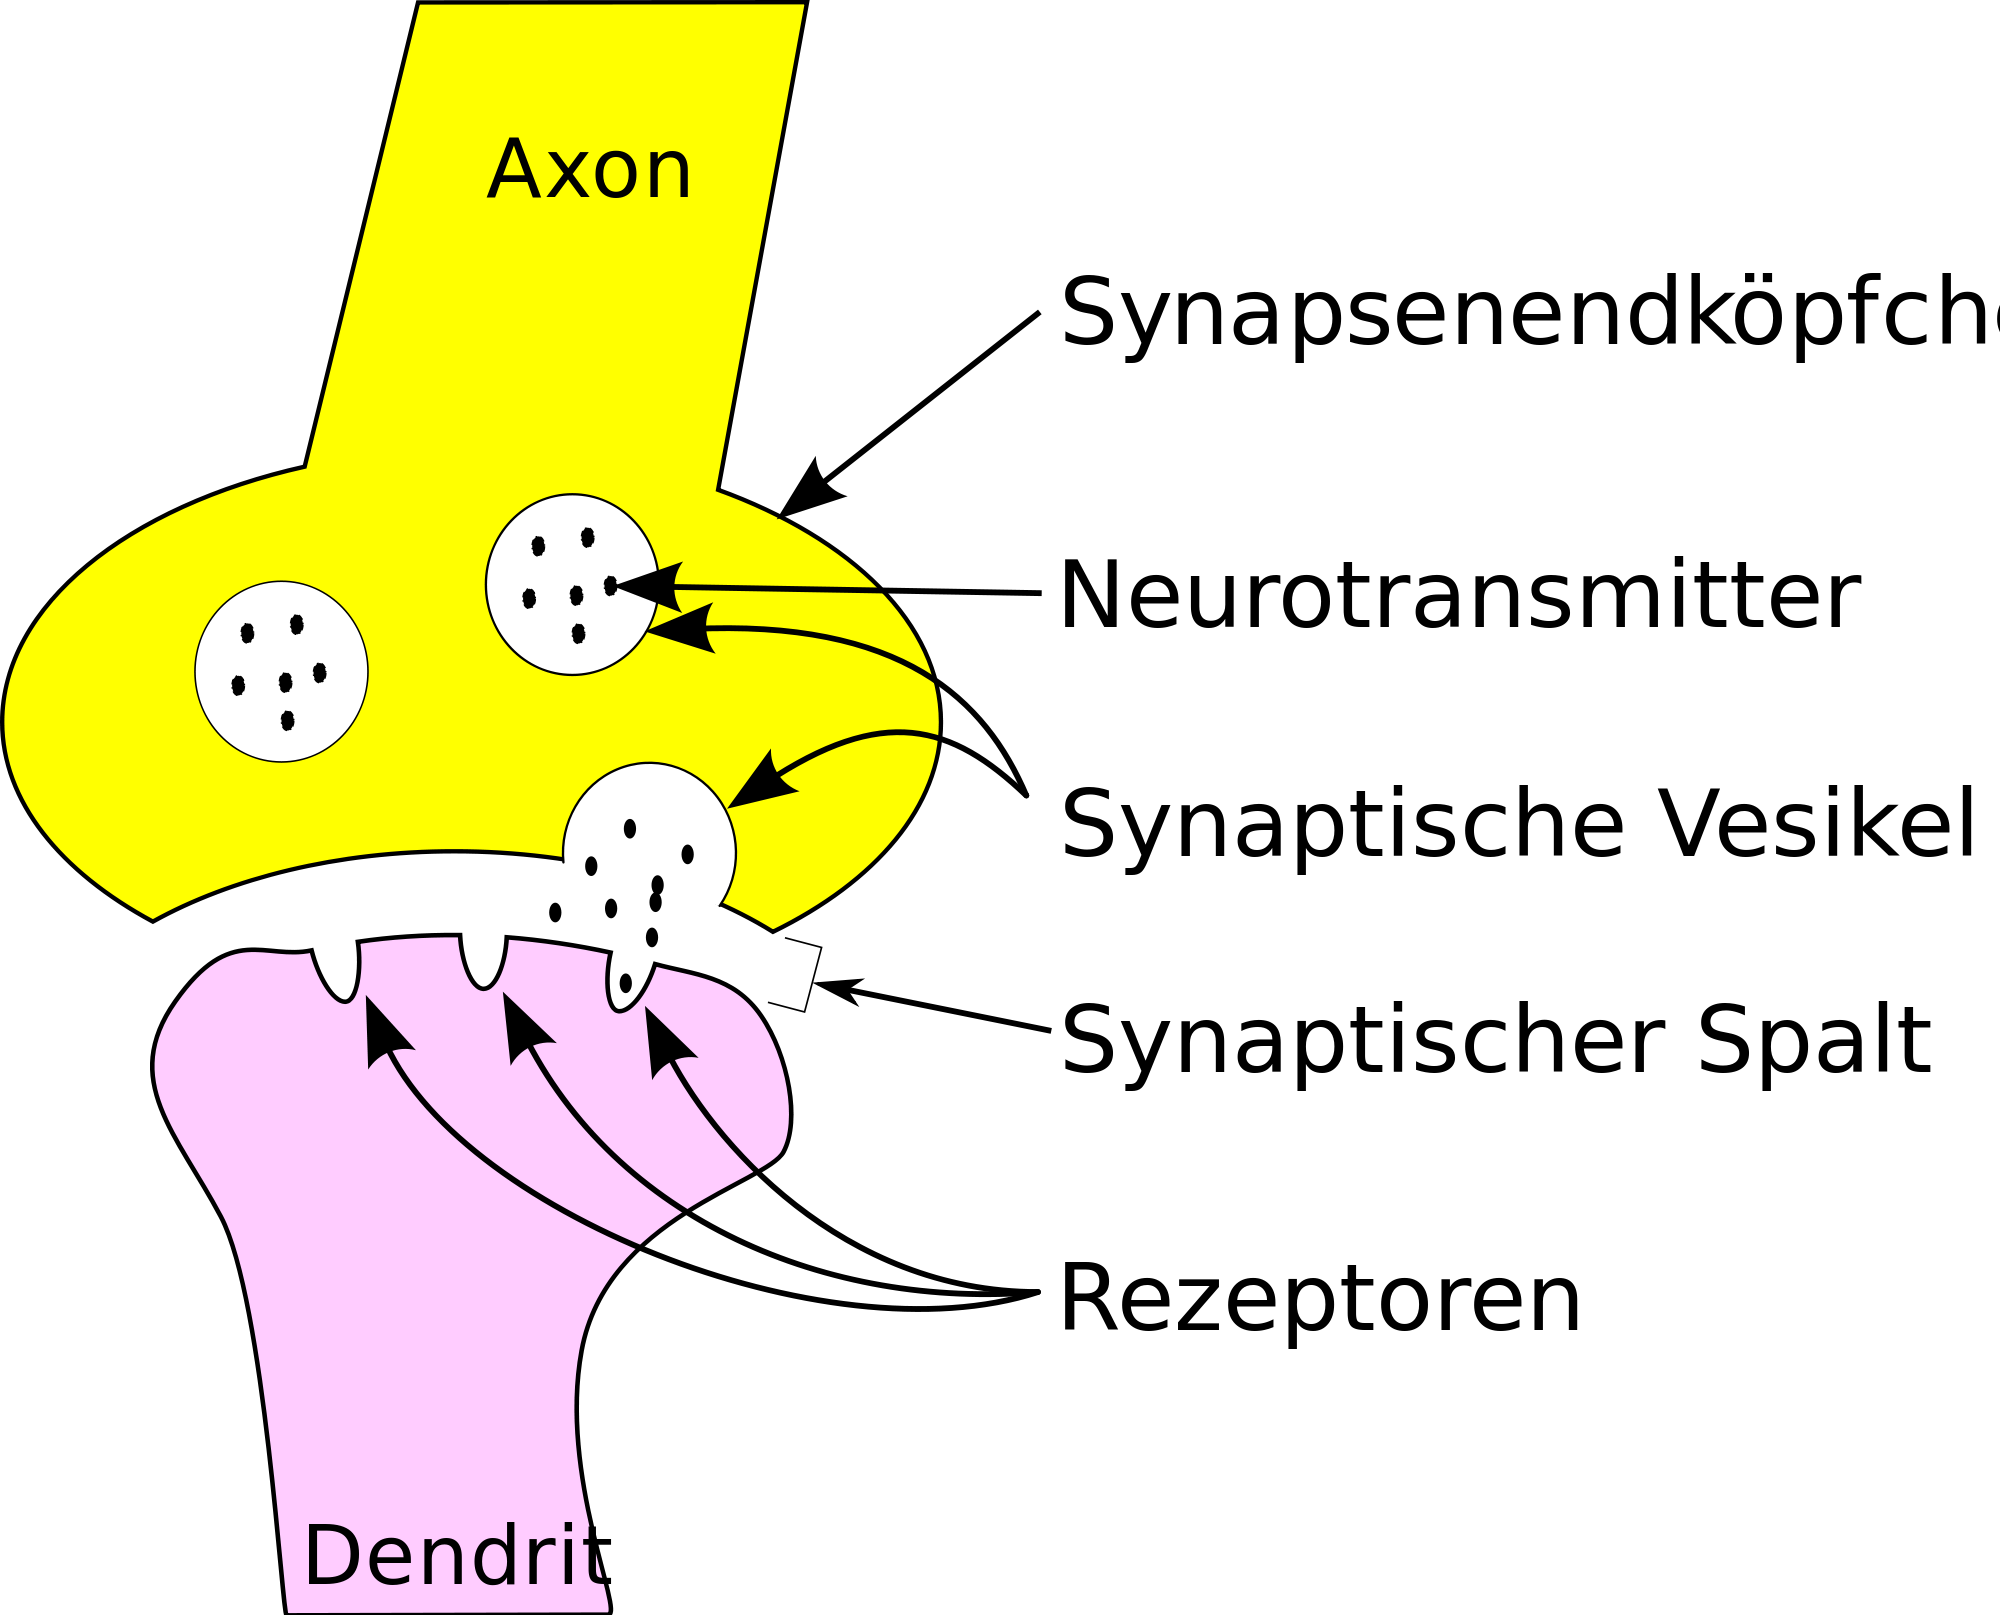
\includegraphics[width=0.35\textwidth]{abb/synapse.png}
	\caption{Abbildung einer Synapse}
\end{wrapfigure}
Wie in Abbildung 3 ersichtlich ist, sind die prä- und postynaptische Zelle nicht direkt miteinander verbunden. Aktionspotentiale werden deshalb, über den sogenannten Synaptischen Spalt, via chemischer Übertragungsweiterleitung propagiert. Gelangt ein Aktionspotential in die präsynaptische Zelle, werden Neurotransmitter, gekapselt in Synaptischen Vesikeln, von der präsynaptischen Zelle ausgestoßen. Dafür verschmelzen die Vesikel mit der Zellmembran, um ihren Inhalt in den synaptischen Spalt zu entleeren. Nach diesem Prozess, der Exozytose genannt wird, diffundieren die Transmitter zu Rezeptoren der postsynaptischen Zelle und binden an Ionenkanäle, was zu einem Influx von Ionen und folglich zu einer Änderung des Membranpotentials der postsynaptischen Zelle führt, auch Postsynaptisches Potential genannt.
\subsection{Neuronale Netze}
Neuronale Netze sind biologisch inspirierte Programmierparadigma, welche es erlauben, iterativ vom Betrachten von Daten zu lernen. Dazu benötigen sie kein domänenspezifisches Wissen, sondern "lernen" Strukturen in den betrachteten Daten selbst zu erkennen. Die Grundeinheit solcher Netzwerke sind dabei künstliche Neuronen, die ihrem biologischen Vorbild aus \ref{sec:neurons} nachempfunden sind. Ein Neuron erhält dabei Eingaben, summiert diese und propagiert einen Wert an andere Neuronen weiter. Dabei kann eine Aktivierungsfunktion eingesetzt werden, die dem biologischen Vorbild der Schwellenwertfunktion ähnelt. Enthält das Neuron also genügend große Eingänge, simuliert es ein Aktionspotential und erzeugt dabei eine Ausgabe. Aufgrund von mathematischer Einfachheit wird die Schwellenwertfunktion in der Praxis durch differenzierbare Funktionen, wie die Logistische Funktion\footnote{$f(x) = \frac{L}{1+e^{-k(x-x_0)}}$}, approximiert. Die Ausgaben solcher Neuronen werden mit Gewichten bewertet, die entscheiden, wie viel des Outputs eines Neurons an seine entsprechenden Nachfolger propagiert wird. Formal lässt sich ein Neuron also als Funktion seiner Eingaben $E$ wie folgt darstellen $$n = f\left(\sum_{i\in E} x_i\right)$$\\
Die simpelste Form eines Neuronalen Netzes ist ein einfaches Perzeptron, welches 1958 von Frank Rosenblatt in \cite{rosenblatt1958perceptron} vorgestellt wurde. Dieses basiert auf einer McCulloch-Pitts-Zelle, einem rudimentären Modell einer Nervenzelle nach \cite{mcculloch1943logical}, enthält mehrere Eingaben und produziert eine einzige Ausgabe. Perzeptrons können prinzipiell aus mehreren Schichten solcher Zellen bestehen, die in Reihe geschaltet sind. Dabei gibt eine Zelle ihren berechneten Output an ein Neuron der nächsten Schichten weiter. Solche Netzwerke heißen Multi-Layer-Perzeptron, im weiteren beschäftigen wir uns jedoch mit einer einzigen Zelle.
\begin{figure}[!h]
	\centering
	\begin{tikzpicture}
	\node[functions] (center) {f};
	\node[below of=center,font=\scriptsize,text width=4em]{};
	\node[right of=center] (right) {};
	\path[draw,->] (center) -- (right);
	\node[functions,left=3em of center] (left) {$\sum$};
	\path[draw,->] (left) -- (center);
	\node[weights,left=3em of left] (2) {$w_3$} -- (2) node[input,left of=2] (l2) {$x_3$};
	\path[draw,->] (l2) -- (2);
	\path[draw,->] (2) -- (left);
	\node[below of=2] (dots) {$\vdots$} -- (dots) node[left of=dots] (ldots) {$\vdots$};
	\node[weights,below of=dots] (n) {$w_n$} -- (n) node[input,left of=n] (ln) {$x_n$};
	\path[draw,->] (ln) -- (n);
	\path[draw,->] (n) -- (left);
	\node[weights,above of=2] (1) {$w_2$} -- (1) node[input,left of=1] (l1) {$x_2$};
	\path[draw,->] (l1) -- (1);
	\path[draw,->] (1) -- (left);
	\node[weights,above of=1] (0) {$w_1$} -- (0) node[input,left of=0] (l0) {$x_1$};
	\path[draw,->] (l0) -- (0);
	\path[draw,->] (0) -- (left);
	\node[below of=ln,font=\scriptsize] {Input};
	\node[below of=n,font=\scriptsize] {Gewichte};
	\end{tikzpicture}
	\caption{Ein einfaches Perzeptron mit n Eingängen}
\end{figure}
Das einfache, in Abbildung 1 dargestellte Perzeptron erhält n Eingänge $x_1,...,x_n \in \mathbb{R}$, die jeweils mit korrespondierenden Gewichten $w_1,...,w_n \in \mathbb{R}$ multipliziert werden. Die Summer der Gewichteten Eingänge wird dann als Argument der Aktivierungsfunktion verwendet. Die Ausgabe des Perzeptron lässt sich als eine Funktion seiner Eingaben wie folgt beschreiben:
\begin{align*}
	\mathbb{P}(\boldsymbol{x}, \boldsymbol{w}) = f(\sum_{i=1}^{n}w_ix_i)
\end{align*}
mit der Aktivierungsfunktion
\begin{align*}
	f(x) = \begin{cases} 1 &\mbox{if } x \geq 0 \\ 
	0 & \mbox{if } x < 0 \end{cases} 
\end{align*}
womit die Ausgabe als Zugehörigkeit zu einer klasse, entweder 0 oder 1 zu interpretieren ist.
\subsection{Convolutional Neural Networks}
Convolutional Neural Networks (CNN) oder Faltungsnetze sind eine Subklasse von Neuronalen Netzen. Sie besitzen also wieder erlernbare Gewichte und Biase. Jedes Neuron erhält eine Reihe Inputs, summiert diese und wendet eine Aktivierungsfunktion darauf an. Der Unterschied zur feedforward Architektur aus dem vorigen Abschnitt besteht darin, dass sie sich die mathematische Operation der Faltung zunutze machen. CNNs wurden in den letzten fünf Jahren besonders in der Bilderkennung äußert erfolgreich angewendet und sind ursprünglich in \cite{lecun1998gradient} dokumentiert, wurden jedoch erst 2012 durch Alex Krizhevsky bekannt gemacht, weil dieser die damalige ImageNet Challenge \footnote{http://www.image-net.org/challenges/LSVRC/} gewann und seine Vorgehensweise in \cite{krizhevsky2012imagenet} beschrieb. Sie besitzen Neuronen, die individuell nur auf Teile des rezeptiven Felds reagieren und orientieren sich so am Aufbau des Visuellen Cortex von Tieren \cite{matsugu2003subject}. Die rezeptiven Felder verschiedener Neuronen überlappen und decken somit das gesamte Visuelle Feld ab. 
\begin{figure}[h!] 
	\centering
	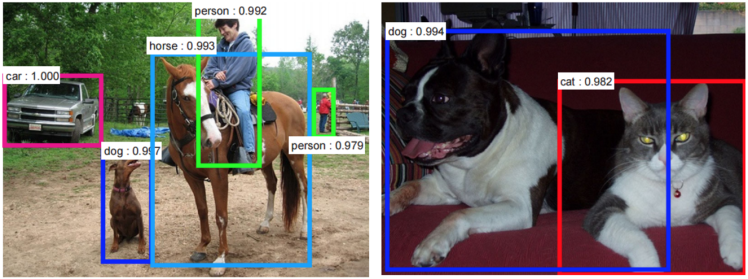
\includegraphics[width=0.7\textwidth]{abb/classification.png}
	\caption{Ein CNN klassifiziert mehrere Objekte pro Bild korrekt mit hoher Konfidenz}
	\label{https://arxiv.org/pdf/1506.01497v3.pdf}
\end{figure}
\subsubsection{Architektur}
CNNs bestehen prinzipiell aus vier Operationen:
\begin{enumerate}
	\item Convolutions
	\item Pooling
	\item Nonlinearities
	\item Classification
\end{enumerate}
Faltungs-, Pooling- und Klassifikations-Layer können dabei beliebig gestapelt werden, um tiefe Architekturen zu erhalten. 
\begin{figure}[h!] 
	\centering
	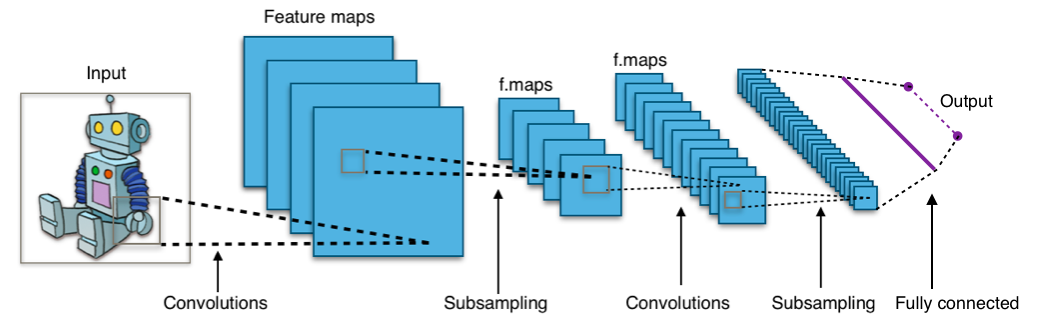
\includegraphics[width=0.7\textwidth]{abb/cnnwp.png}
	\caption{Beispielhafte Architektur eines CNNs. Subsampling steht hierbei für Pooling-Layer.}
	\label{fig1}
\end{figure}
\clearpage
\subsubsection{FaltungsLayer}
\begin{wrapfigure}{R}{0.4\textwidth}
	\centering
	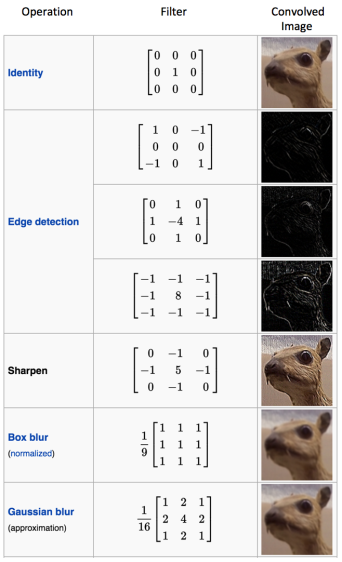
\includegraphics[width=0.35\textwidth]{abb/convolution.png}
	\caption{Verschiedene Faltungskernel}
\end{wrapfigure}
Konvolutionslayer bestehen aus einer Reihe lernbarer Filter. Filter sind kleine Matrizen, die im Rahmen der Konvolution benutzt werden. Im Folgenden werden Filter der Größe 3x3 Pixel verwendet. Während der Netzwerkpropagation werden die Filter über das Eingangsbild des Layers geschoben und die einzelnen Filterwerte mit den korrespondierenden Pixeln des Bilds multipliziert. In jeder Position wird dann der Mittelwert berechnet und daraus eine sogenannte Feature Matrix gebildet. Sind mehrere Filter pro Layer vorhanden, wird dieser Schritt für jeden vorhandenen Filter wiederholt. Beim Training lernt das Netzwerk, Filter zu bilden, die Kanten bestimmter Ausrichtung erkennen können.
Der Namensgeber dieser Netzwerke ist die mathematische Faltung, deren Aufgabe es in diesem Kontext ist, Muster in den Daten aufzudecken. Für den diskreten, zweidimensionalen Fall ist die Faltung $\textit{\textbf{f}}, \textit{\textbf{k}}: \mathbb{R}^n\times\mathbb{R}^n \rightarrow \mathbb{R}$ formal mit
$$ \textbf{I}^*(x, y) = \sum_{i=1}^{n}\sum_{j=1}^{n}\textbf{I}(x+i-a, y+j-a)k(i,j) $$
gegeben, wobei $\mathbb{I}$ das Eingangsbild, $a$ die Koordinate des Mittelpunkts der quadratischen Faltungsmatrix, und $k(i,j)$ einem Element der Faltungsmatrix $k$.
\subsubsection{Pooling-Layer}

\subsection{Rekurrente Neuronale Netze}
Rekurrente Neuronale Netze (RNN) sind eine Subklasse Neuronaler Netze, in denen gerichtete Kreise vorhanden sind. Dies führt dazu, dass die Netze einen internen Status besitzen, der ihnen erlaubt, temporales Verhalten abzubilden. So können sie sich beispielsweise ihre Aussage aus der Vergangenheit merken und somit zukünftige Ergebnisse beeinflussen.\\
Im Gegensatz zu feedforward Netzen, die ihren Informationen vom Input zum Output propagieren, sind RNNs also zusätzlich von Informationen aus früheren Phasen abhängig. Dies führt dazu, dass sie bei Training und Analyse nicht wie feedforward Netze behandelt werden können, was Arbeiten mit ihnen in einigen Fällen erschweren kann. In vielen Fällen wird Systemtheorie verwendet, um RNNs zu verstehen, jedoch wird in dieser Arbeit eine Approximationsmethode benutzt, die es erlaubt, Techniken für feedforward Netze auch für RNNs zu benutzen.
\subsection{Approximation von Rekursion}
Um RNNs mit den Methoden des Deep Learnings zu benutzen, können sie über Zeitschritte entfaltet werden. Dabei erhält meine eine feedforward Architektur, die in einem Rechenschritt die Eingänge mehrerer Zeitschritte erhält und diese im Netzwerk berücksichtigt. 
\begin{figure}[h!] 
	\centering
	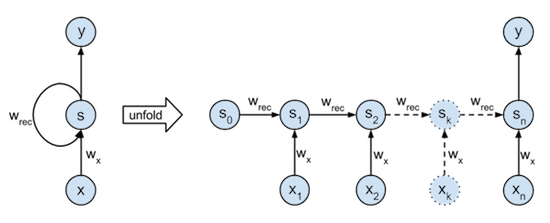
\includegraphics[width=0.7\textwidth]{abb/rnn.png}
	\caption{Ein RNN wird über n Zeitschritte entfaltet. Die Netzwerkeingaben $x_1,..., x_n$ müssen hierbei alle zur Verfügung stehen.}
	\label{img:rnn}
\end{figure}
Die Güte der Approximation hängt von der Anzahl der gewählten Zeitschritte ab. Je mehr Zeitschritte hier berücksichtigt werden, desto besser approximiert das Netzwerk. Jedoch besteht bei hohen $k$ die Gefahr von verschwindenden oder explodierenden Gradienten. Da häufig verwendete Aktivierungsfunktionen wie der tangens hyperbolicus\footnote{$y = tanh\ x = \frac{sinh\ x}{cosh\ x} = \frac{e^x - e^{-x}}{e^x + e^{-x}}$} Die Gewichte $w_{rec}$ und $w_x$ werden dabei über Zeitschritte geteilt und der Netzwerkfehler ist der Durchschnitt der Fehler der einzelnen Zeitschritte. 
\subsection{Backpropagation} 
Backpropagation is a widely used technique to train neural networks. It is, in fact, the algorithm that made training deep neural networks tractable in the first place. While being originally introduced in the 1970's it has not been adapted until David Rumelheart, Geoffrey Hinton and Ronald Williams drew a lot of attention to it in their famous 1986 Paper \cite{rumelhart1988learning}. At the core of Backpropagation stand partial derivatives like $\frac{\delta C}{\delta w}$ of a cost function C with respect to a weight w. This gradient expresses, at what rate C changes if we tune w. Knowing how the error of the network behaves when changing a parameter can be very helpful, since we then can adjust it in a way, such that our total error decreases.
In order to minimize our cost function we therefore have to compute the partial derivatives of the networks cost function with regard to every variable in the network i.e. every weight and bias. We then use those gradients to move "downwards" on our cost function i.e. adding a small positive value to our weight or bias, if the gradient is negative and vice versa adding a small negative value, if the gradient is positive.
\\
\begin{tikzpicture}[>=stealth, every node/.style={circle, draw, minimum size=0.75cm}]
\graph [tree layout, grow=down, fresh nodes, level distance=0.5in, sibling distance=0.5in]
{
	g = e * f <- { 
		e = a + b <- { a, b },
		f = 3 * c <- { c }
	} 
};
\end{tikzpicture}
\subsection{Backpropagation Through Time}